\documentclass[11pt]{article}

\usepackage{sectsty}
\usepackage{graphicx}
\graphicspath{ {./static/} }

% Margins
\topmargin=-0.45in
\evensidemargin=0in
\oddsidemargin=0in
\textwidth=6.5in
\textheight=9.0in
\headsep=0.25in

\title{ VR Project}
\author{ Arnav Rustagi}
\date{\today}

\begin{document}
\maketitle	
\pagebreak

% Optional TOC
\tableofcontents
% \pagebreak

%--Paper--

\section{Question 1}

\subsection{Transformations}
\subsubsection{Translation}
\begin{center}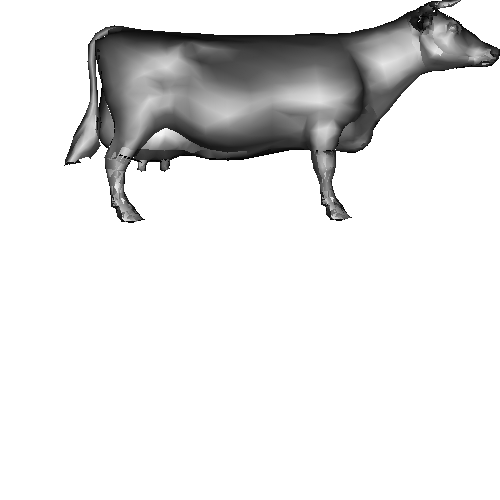
\includegraphics{translation}\end{center}
\subsubsection{Rotation}
\begin{center}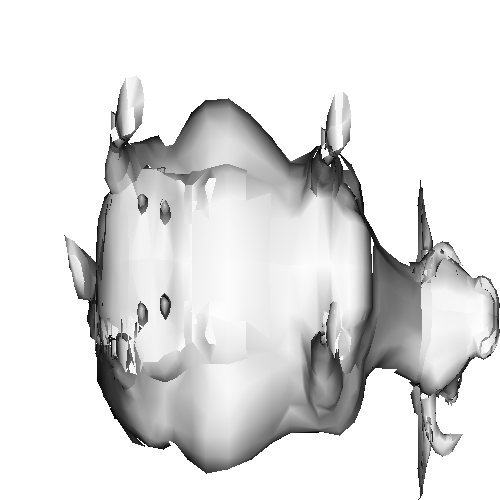
\includegraphics{rotation}\end{center}
\subsubsection{Scale}
\begin{center}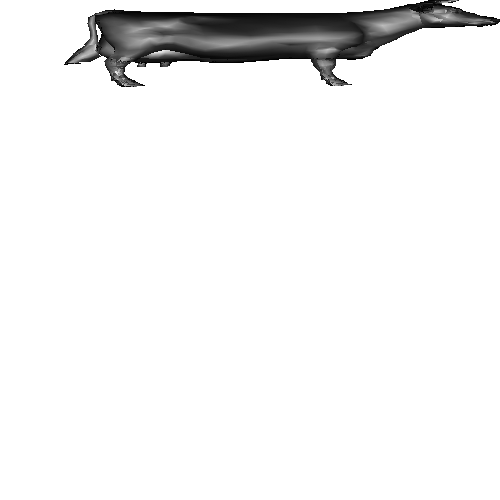
\includegraphics{scale}\end{center}
\subsection{Everything}
\begin{center}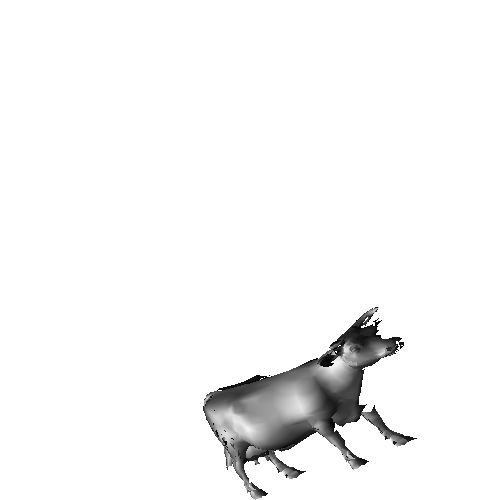
\includegraphics{q1}\end{center}


\pagebreak
\section{Question 2}
Simple Dead Reckoning often has errors attributed to the tilt axis being misplaced, these errors are called tilt errors, and cause the headset to slowly drift away from the actual orientation of the headset.\\\\
This is often fixed by applying a tilt axis rectification function, which rectifies the tilt axis, this significantly reduces the tilt error\\\\

I am not sure if my data is correct as I feel i made an error in how I assesed and fixed the tilt error, and I have also not implemented some utility to graph the said graph
\pagebreak
\section{Question 3}
\subsection{Simple Dead Reckoning}
This method has a time complexity of $O(N)$ as the quaternion multiplication is of constant time, given the constant dimension of the quaternion, and the rest of the operations are also constant time. Here $N$ stands for the length of the input data
\subsection{Dead Reckoning with Tilt Correction}
This method also has a time complexity of $O(N)$ as all the operations are  the same, the only difference being you have to iterate through the whole array again, this doubles the time complexity, but we do not account for it in the big O notation.
\subsection{Conclusion}
We can say that both these functions are similar in time complexity, but the second method has better results, so overall the second method is preffered, as it actually ensures that the product works the way it is intended
\pagebreak
\section{Question 4}
The positional tracking is posible as quaternions tell us how the headset is oriented. Potential limitations might be translatory motion as the IMUData does not contain sensor data for translatory motion, which is often a feature which is supported by modern headsets
\pagebreak
\section{Question 5}
The problem with colision polygons being spheres is the fact that the colisions are not limited to the geometry of the objected, often in games you want different shapes of collisions to not only tell the rendering engine how the geometry of the given model works, but often to show several things like hitboxes, collisions with different objects in the world.\\\\
Not generalising every collision polygon as a sphere gives the developer more freedom on how he/she wants the model to interact with the world, a good example could be a boss' hitbox, which the developer might want to be hidden beneath a thin arm, this arm nor the hitbox can have a spherical hitbox
\pagebreak
\section{Question 6}
The distortion correction can be implemented in a GPU by using transformation matrix' as GPUs excel at doing matrix multiplication, an easy way is that of multiplying every position $(x,y)$ with a transformation matrix to move it to its new position $(xnew,ynew)$.\\\\
Another ambitious idea might be to create a new matrix of the same dimensions as the image, and multiply it with the image, but I am not sure about its feasability, or the maths adding up

%--/Paper--

\end{document}
